\documentclass[titlepage]{article}
\usepackage[bottom=3cm, right=3cm, left=3cm, top=3cm]{geometry}
\usepackage {graphicx}
\usepackage{caption}
%opening
\title{%
	Practical Machine Learning\\
	
	\vspace*{2em}
	\LARGE Exercise 4\\
	Spring 2024}
\author{Lisa Stafford}
\date{March 15, 2024}

\begin{document}
	\setlength\parindent{0pt}
	
	\maketitle
	
	\section*{Abstract}
	Hyper-parameter selection is a common problem for machine learning architects where one selects the model that does the best job of generalizing and most appropriate for the given problem, but without proper knowledge of hyper-parameters within the model and what they actually do to affect the model performance, many users new to machine learning may be unaware how to select or tune hyper-parameters correctly, and most non-data scientists don't know (or may not be aware of without significant trial and error) how those hyper-parameters affect the overall runtime and performance of their model.  After selecting a base model, hyper-parameter selection remains an important part of the machine learning process.  
	
	\section*{Introduction}
	In order to learn and determine which hyper-parameters have the greatest overall effect upon the model run-time, resource use, and performance, we seek to isolate hyper-parameter selection by isolating variables in which to evaluate the performance, resource use, and runtime without changing underlying factors that may also affect model performance.  Throughout our investigation, we used a wine data set obtained from the University of Irvine \cite{dataset}. Training is performed on only the white wine within the data set.  Several models are trained implementing hyper-parameter optimization libraries directly from scikitlearn \cite{scikitlearn} and then obtaining total runtime, and training and testing performance scores and tuned hyper-parameter choices for a number of hyper-parameter tuning mechanisms.  
	
	\section*{Dataset Description}
	Our wine data set is actually comprised of two different wine subsets of data.  While both are related to variants of \cite{dataset} "Portuguese Vhinho Verde wine" the data is actually split in two subsets - one red subset and one white subset.  In this exercise, we will only be performing machine learning tasks on the white wine data set since the parameter tuning time should be extensive for each run, and instructions indicate we must not be able to use a grid search on the hyperparameter space.  All wine subset contains 11 features and 1 label for wine quality.   All features are continuous float values.  Within the model the "wine quality" labels are recognized as discrete categorical integer values ranging from 3 to 9 for the white wines.  White wine contains a total of 4898 total data instances, as shown in the following table images. Figure 1 displays feature values, statistics, and total instances for white wine.  The image to the right shows feature correlation to the output label.  
	
	\begin{center}
		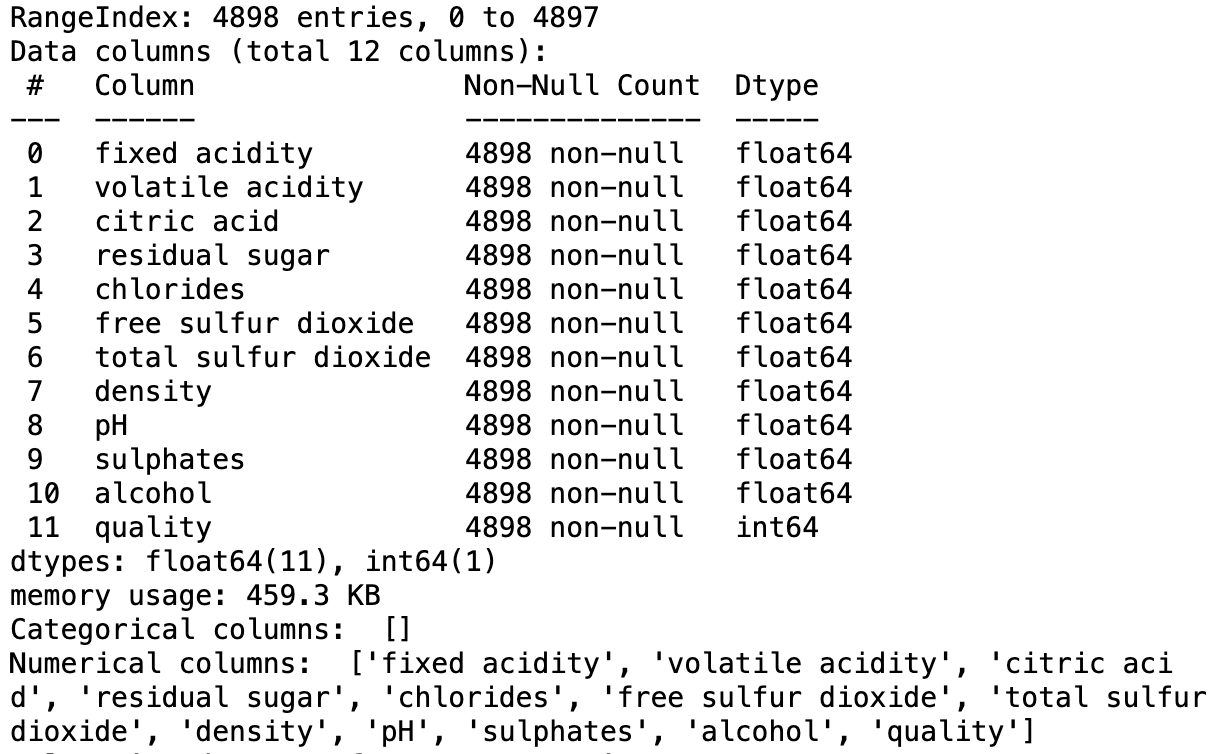
\includegraphics[width=.55\textwidth]{img/white.png}
		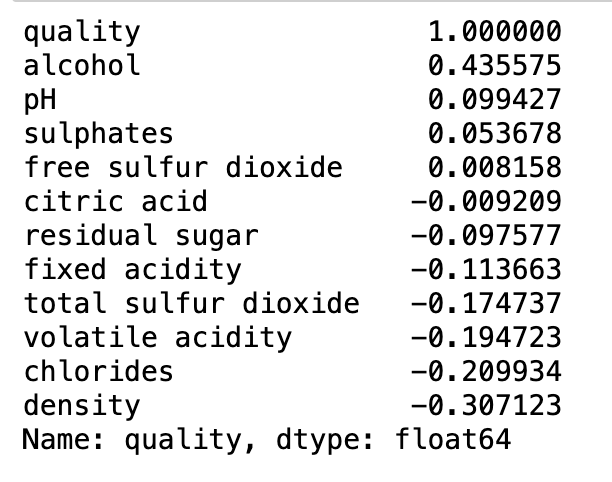
\includegraphics[width=.405\textwidth]{img/ww_feature_correlation.png}
	\end{center}

	\noindent As mentioned from prior exercises, white wine data is somewhat "pre-cleaned".   The feature values are all continuous and contain no missing data values, however these features are not evenly distributed.  The data values are somewhat bell-shaped with a larger number of data instances with labels closer to the mean.  As described on the data set website \cite{dataset} both "data set... classes are ordered and []unbalanced] so there are many more normal wines than excellent or poor ones.... [also], both datasets have 11 physiochemical features... and a sensory output label, ('quality')".   The following histogram shows the distribution of class instances within the dataset:  
	
	\begin{center}
		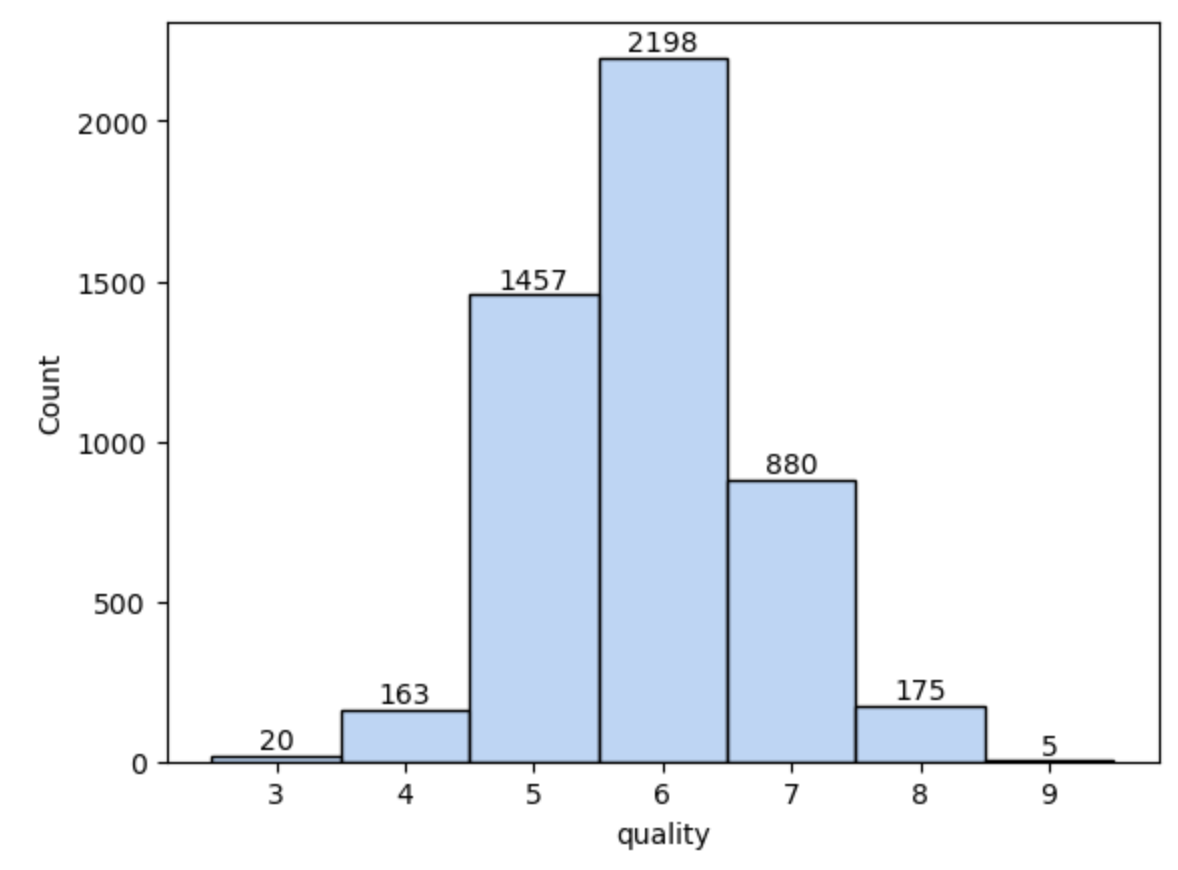
\includegraphics[width=.55\textwidth]{img/ww_data_distribution.png}
	\end{center}
	
	Standard Scaling worked best as a data transformation method in Exercise 2, so we will use it in this exercise since we would like to automate and optimize our performance on a Random Forest Classifier from the ensemble library in ScikitLearn \cite{scikitlearn} and K-Nearest Neighbors classifier from the neighbors library.  Though the whole of the search relies on a decision tree, sub-estimators are reliant on other classifiers like SVMs which have been shown in previous exercises to be sensitive to unscaled data.  We want to experiment with subsets of most important features obtained from an updated version of our data set exploration exercise since this could have significant impact on overall performance for any classifier.  The Random Forest Classifier also automates feature correlations noted in a prior chart when deciding which features to extract or drop or group from the dataset per it's 'max\_features' parameter which we'll set as a hyperparameter for optimization.  Overall, dropping unimportant or redundant features will not only help with the speed at which the model optimization completes, it may also provide better performance if the features are not that important in label prediction, and may help performance if the feature is redundant or very similar to another feature already contained within the dataset.  This would need to be programmed into capabilities for k-neighbors.  
	
	\section*{Experimental Setup}
		We are looking at the wine quality data set, specifically, the white wines in the data set.  From there, we're trying to predict wine quality for items within the data set to determine the best hyper-parameters and methods for finding them are done so in the most optimized way.  
		
		\vspace{.2cm}
		We know that this particular data set is supervised and the problem is a classification problem with a known number of categories. Therefore we know that the best ML models will be in that realm.  In prior exercises Random Forest Classifiers and KNN worked best and most consistently therefore we will attempt to optimize the hyperparameters for these 2 classification model types.  We have a large number of hyperparameters to search through given the two model options. For larger continuous hyperparameters, we will iterate through certain values manually selected.  Method of optimizing our hyperparameters will include:  
	\begin{enumerate}
		\item Initially perorming a Randomized Search with 5-Fold Cross Validation ($RandomizedSearchCV()$) on the model and listed hyperparameters in order to pre-find some hyperparameters that perform well.  This should be easy to do since the $RandomizedSearchCV()$ appears to take much less time on average than other hyperparameter optimization searchers.  On average, the Random search optimizer takes around 1 minute to complete, therefore we will run it 10 times and see if we can note any patterns.  
		\item Attempting (but possibly failing) when pretuning Hyperparameters (Metalearning) by finding an initial list of the best subsets of hyperparameters by performing a 5-Fold Cross Validated Grid Search ($GridSearchCV$) on hyperparameters to find those that perform most optimally on smaller subsets of the dataset.  This may fail because the algorithm for grid search may still be too complex and time consuming to perform, even on a smaller dataset. 
		\item Running the out of the box Bayesian Search with 5-Fold Cross Validation ($BayesSearchCV()$) available in the skoptimizer library.  
	\end{enumerate}
	
	Searchers were conducted on a list of classifier hyperparameters populated from a python $dict()$ as follows.  
	\vspace{.3cm}
	\newline\textbf{Random Forest Classifier Hyper-parameter Options (left): KNN (right) } \newline
	\begin{tabular}{l l}
		\begin{tabular}{ l | l }
			\textbf{n\_estimators:} & 50, 100, 200, 300  \\
			\textbf{criterion:} & 'gini', 'entropy', 'log\_loss'  \\
			\textbf{max\_depth:} & None, 15, 25, 50   \\
			\textbf{bootstrap:} & True, False \\
			\textbf{min\_samples\_split:}  & 5, 10  \\
			\textbf{min\_samples\_leaf:} & 1, 2, 5 \\
			\textbf{min\_weight\_fraction\_leaf:} & 0.001, 0.01, 0.1  \\
			\textbf{class\_weight} & 'balanced', 'bal\_sub \\
			\textbf{max\_features:} & 'sqrt', 'log2', None \\
			\textbf{n\_jobs: } & -1 \\
		\end{tabular}  &
		\begin{tabular}{ l | l }
			\textbf{n\_neighbors:} & 2,5,10,25,50  \\
			\textbf{weights:} & uniform, distance  \\
			\textbf{algorithm:} & ball\_tree, kd\_tree, auto   \\
			\textbf{leaf\_size:} & 5,10,15,20,30,40,50 \\
			\textbf{n\_jobs: } & -1 \\
		\end{tabular} \\
	\end{tabular}
	\vspace{.3cm}\newline
Since the RandomSearchCV for hyperparameter optimization performs very quickly (our average run for a Random Search is under 1 minute), we use it as a base with our full dataset to get a very general idea of which hyperparameters perform the best by running it over 10 iterations and reporting resulting "best hyperparameters".   After only a few runs, it becomes very clear that certain hyperparameter settings (such as setting minimum sample leafs to anything over 2 or min\_weight\_fraction\_leaf over .1) resulted in a vastly worse model and notable drop in accuracy scores.    Similar performance is noted with KNN for all less common classes within the dataset, but also an overall lack of accuracy was noted for KNN. Examples of improper fits are shown below for Random Forest on the left and KNN on the right:  
\begin{center}
	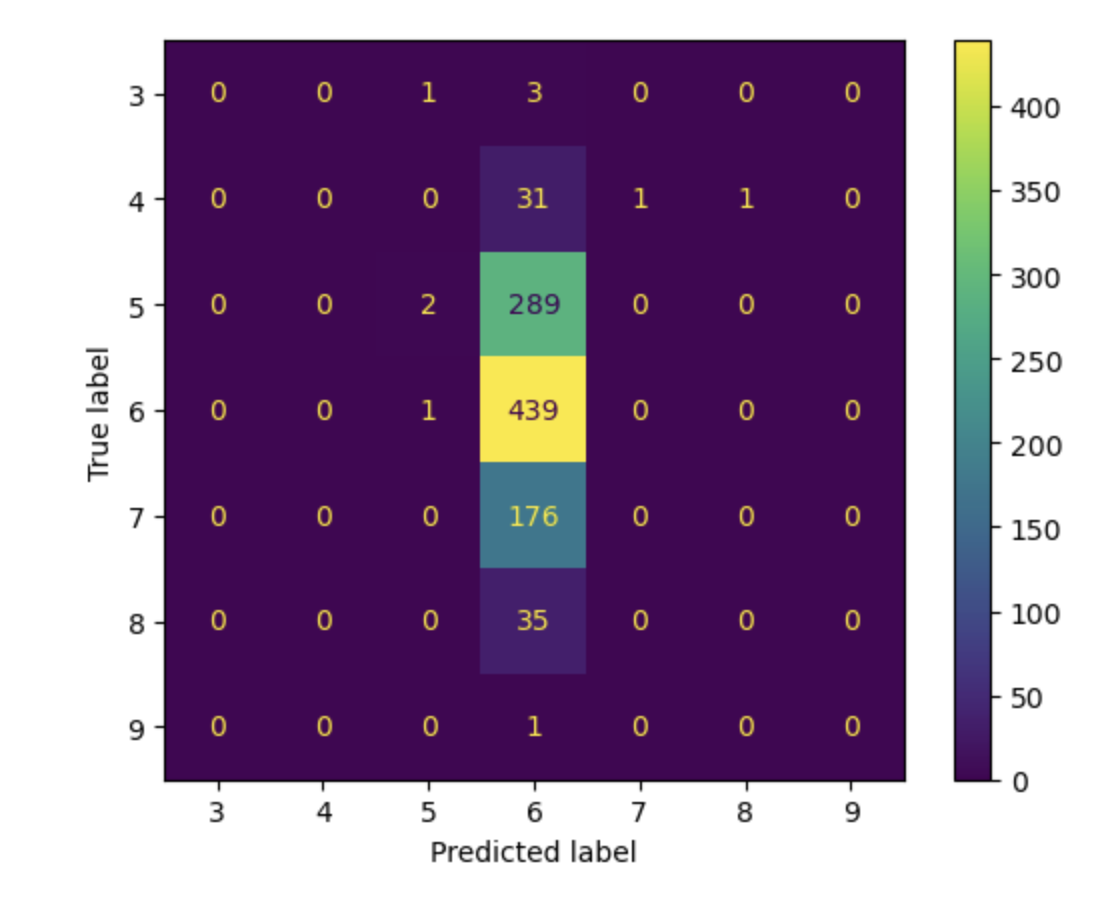
\includegraphics[width=.42\textwidth]{img/garbage.png}
	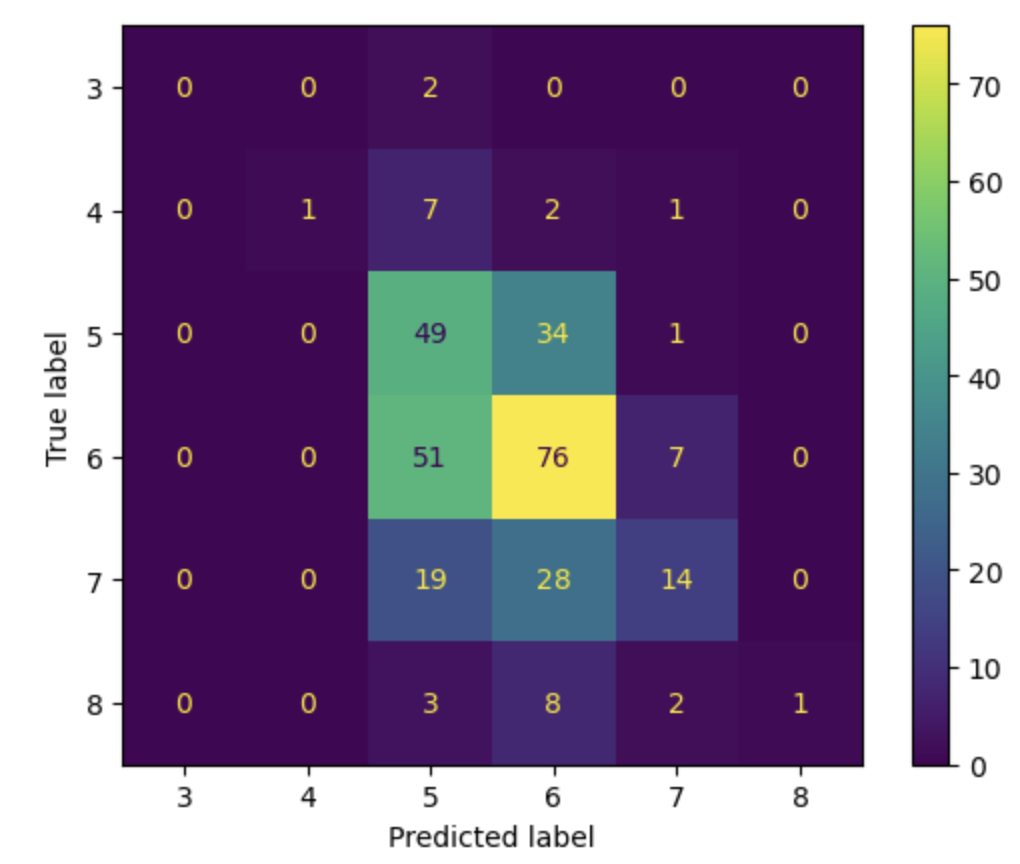
\includegraphics[width=.4\textwidth]{img/knngarbage.png}
\end{center}

The resulting performance when setting sample leafs to higher values is now obvious in hindsight.  This is because several outlier label classes (like class 3 or class 9) had very few instances to begin with and therefore the model becomes extremely biased towards the most commonly "seen" labels (in this dataset, that's wine qualities 5 and 6).  For RandomForestClassifier(), Setting the min\_sample\_leaf to anything over 5 or min\_weight\_fraction\_leaf over .1 will result in the uncommon classes simply being disregarded as a possibility.  Therefore these options are completely removed before running any further hyperparameter tuning.  Since the overall performance shown between these two models seems to be more consistent and promising with Random Forest Classifiers, we proceed with this particular model, and pitch our work on the KNN model.
\vspace{.2cm}\newline
To follow up, we attempt to perform a grid search upon a subset of data beginning with a 25\% random sample.  It is in hopes that this will help us gain more information through "metalearning".  Unfortunately, this fails to pay off, as the grid search never completes, despite only being fed 25\% of the total dataset.  We again attempt to metalearn with the smaller red wine dataset since it has 1600 instances instead of the white wine's 4900, however this also fails to complete.  The total number of hyperparameters in our search space is simply too large, regardless of the total number of instances in the dataset.  Therefore, we attempt metalearning again using the bayesian search cv library in SciKit-Optimizer \cite{skopt} and again perform the optimization on a 25\% subset of the full white wine dataset.  This metalearning variant of the BayesSearchCV run results in a 58\% accuracy rate with the following recommended hyperparameters:  
\vspace{.2cm}\newline
	\begin{tabular}{ l | l  }
	\textbf{Training Accuracy:} &99.5\% \\
	\textbf{Test Accuracy:} & 58.17\% \\
	\textbf{N Estimators:} &  300  \\
	\textbf{Class Weight:} & Balanced Subsample  \\
	\textbf{Bootstrap:} & True \\
	\textbf{Criterion:}  & Entropy  \\
	\textbf{Max Depth:} & 50\\
	\textbf{Min Sample Leaf:} & 1 \\
	\textbf{Min Samples Split:} & 5 \\
	\textbf{Max Features:} &  log2  \\
	\textbf{Min Weight Fraction Leaf:} &  0.001  \\
	\textbf{N Jobs: } & -1 \\
	\textbf{Fit Runtime:} &  128.78 seconds \\
\end{tabular}
\vspace{.2cm}\newline
While this particular search did not perform well with outlier labels, this is expected, since a subsample of the full dataset will have very few outlier labels available for training.  A confusion matrix for this bayesian search on hyperparameters shows the following performance:  
\begin{center}
	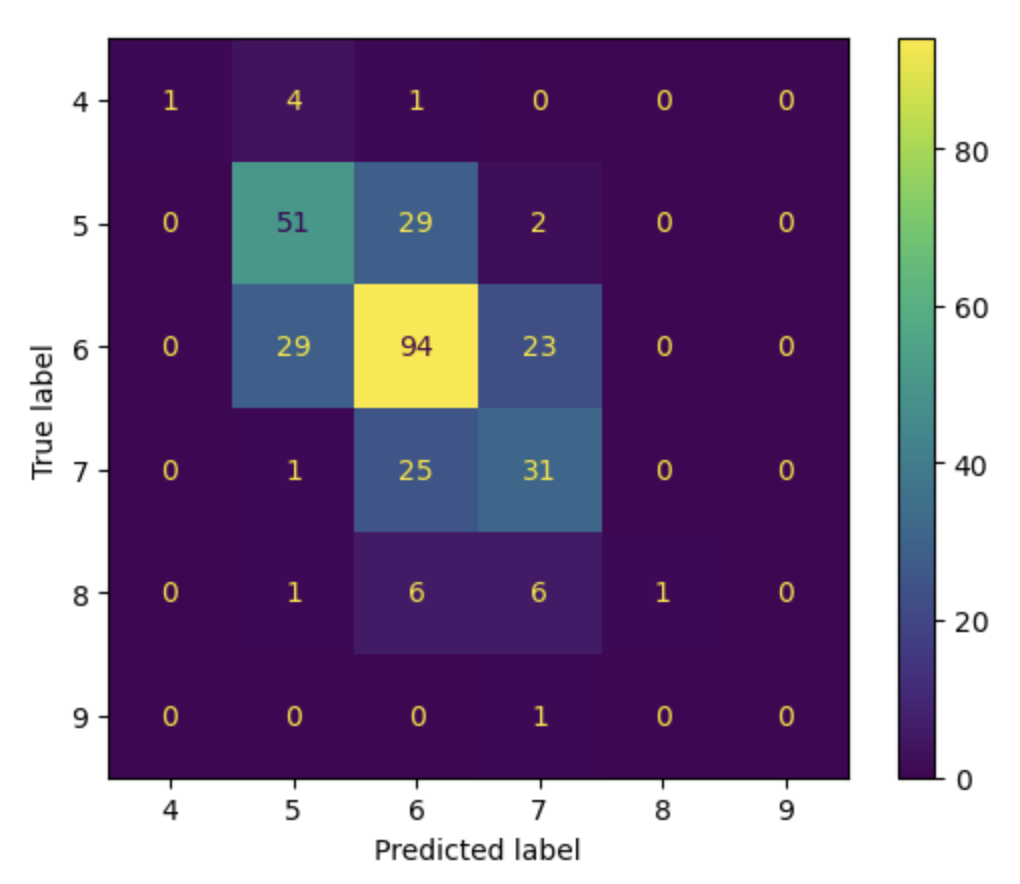
\includegraphics[width=.44\textwidth]{img/bayessearchperf.png}
\end{center}

Given the speed at which this completes, we re-sample the subset of data from the full dataset and perform the same search again over 10 iterations to see if there are any patterns of note.  Over the course of 10 runs we get the following results:  
\vspace{.2cm}\newline
	\begin{tabular}{ l | l | l | l | l | l | l | l | l | l | l }
	\textbf{Run \#:} & 1 & 2 & 3 & 4 & 5 & 6 & 7  & 8 & 9 & 10\\		
	\hline
	\textbf{Train Acc:} & .995 & .995 & .9945 & .993 & .999 & .997 & .997 & .993 & .998 & .997 \\
	\textbf{Test Acc:} & .5817 & .572 & .542 & .621 &  .56 & .6 & .621 & .621 & .56  & .54 \\
	\textbf{\#Estims:} &  300 & 300  & 50 & 100 & 300 & 300 & 300 &  300 & 300 & 300 \\  
	\textbf{Class Wt:} & BS  & BS &  BS & B & BS & BS & BS &  BS &  B &  BS \\
	\textbf{Bootstrap:} & True & " " & " " &  " " & " " & " " &  " " & " " & " " & " "  \\
	\textbf{Criterion:}  & Ent.  & LL &  LL  & Ent & Ent  & LL & Ent & Ent & LL & Ent \\
	\textbf{Mx Depth:} & 50 & 50 & -1 & -1 & 50 & -1 & -1  & 50 & -1 & 50 \\
	\textbf{Min Smpl Lf:} & 1 & 2 & 1 & 1 & 1 & 2 & 2 & 1 & 1 & 1 \\
	\textbf{Min Smpl Split:} & 5 & " " & " " & " " & " " &  " " & " " &  " " &  " " & " " \\
	\textbf{Mx Feat:} & log & $\sqrt{f}$ & log & $\sqrt{f}$ & log & $\sqrt{f}$ & log & $\sqrt{f}$ & $\sqrt{f}$ & $\sqrt{f}$ \\
	\textbf{Min Wt Frac Lf:} &  0.001 & " " & " " & " " &  " " & " " & " " & " " & " " & " " \\
	\textbf{\#Jobs:} & -1  & " " & " " & " " & " " & " " & " " & " " & " " & " " \\
	\textbf{Fit Time (sec:)} &  128.8 & 119.6 & 149.4 &  93.17 & 141.4 & 136.5 & 115.7 & 130.54 & 121.8 & 146.35 \\
\end{tabular}
\vspace{.2cm}\newline
From this we may make some reasonable assumptions:
\begin{enumerate}
	\item We can remove the smallest value from the number of estimators since that never resulted in an optimal score over the course of any of our 10 searches. 
	\item Setting bootstraping to True always resulted in the optimal hyperparameter over the course of 10 searches of the hyperparameter space, therefore we remove the False option (which is the default) and set it to True for all cases.  
	\item The model always performed best when Minimum Weight Fraction Leaf hyperparameter was set to the lowest value so we remove it from our search space since the default for a Random Forest Classifier model will set it to 0.  
	\item The search always found the minimum sample split optimal value to be 5 for all 10 runs, therefore we remove values higher than 5, and add a lower value to see if that results in any change to performance. 
	\item The model always performs better with a higher maximum depth and having it set to None does not appear to have any significant affect on the overall runtime, therefore we remove the hyperparameters from the search space so the model may take simply the default - None.   
\end{enumerate}

After making these changes to our hyperparameter search space, we run 5 runs of our Random Search CV on the new subset.  Two things are notable in the results of our random search:
\begin{enumerate}
	\item Model test accuracy has improved on average from .58 in our original run to .685 in the updated randomized search run.  This is a significant improvement.
	\item Average run time for fitting using randomized search remains around 1 minute or less, so we do not appear to have negatively impacted overall runtime for hyperparameter tuning.  
	\item We have yet to ever see 'gini' criterion perform optimally, despite being the default hyperparameter for the model.  While this is the case, because we don't fully understand the difference between 'entropy' and 'gini' and entropy has performed well in prior instances, we leave it in the search space.  
\end{enumerate}
Given our results and improvements with our updated hyperparameter search space, we perform our bayesian search on our data subsets another 10 iterations, again noting performance.  

\begin{tabular}{ l | l | l | l | l | l | l | l | l | l | l }
	\textbf{Run \#:} & 1 & 2 & 3 & 4 & 5 & 6 & 7  & 8 & 9 & 10\\		
	\hline
	\textbf{Train Acc:} & 1 & .998 & .997 & .99 & 1 & .992 & .999  & .995 & .999 & .998 \\
	\textbf{Test Acc:} & .59 & .575 & .61 & .593 & .595 & .585 & .588 & .628 & .614 & .58 \\
	\textbf{\#Estims:} &  300 & 300 & 100 & 300 & 300 & 300 & 300 & 300 & 300 & 300 \\  
	\textbf{Class Wt:} & BS & B & BS & B & B & BS & B & B & BS & B  \\
	\textbf{Bootstrap:} & True & " " & " " & " " & " " & " " & " " & " " & " " & " "  \\
	\textbf{Criterion:} & LL  & Ent & LL & Ent & Ent & LL  & LL & LL & LL & LL \\
	\textbf{Min Smpl Lf:} & 1 & 2 & 1 & 2 & 1 & 2 & 1 & 2 & 2 & 1 \\
	\textbf{Min Smpl Split:} & 2 & 2 & 2 & 5 & 4 & 5 & 2 & 2 & 5 & 2 \\
	\textbf{Mx Feat:} & $\sqrt{f}$ & log & $\sqrt{f}$ & $\sqrt{f}$ & log & $\sqrt{f}$  & $\sqrt{f}$ & $\sqrt{f}$ & $\sqrt{f}$ & $\sqrt{f}$ \\
	\textbf{\#Jobs:} & -1  & " " & " " & " " & " " & " " & " " & " " & " " & " " \\
	\textbf{Fit Time (sec:)} & 139.46 & 129.04 & 119.8 & 106.5 & 122.56 & 120.22 & 121.61 & 128.46 & 138.9 & 126.11 \\
\end{tabular}
\vspace{.2cm}\newline

This time we don't notice much of a change to performance, nor to runtime.  The number of estimators is mostly consistent with best results using 300 estimators, so we remove the other options from the hyperparameter search space.  With this in place, we can now run the Bayesian Search on the entire dataset. Our final model results in the following for 3 runs:  

\begin{tabular}{ l | l | l | l }
	\textbf{Run \#:} & 1 & 2 & 3 \\
	\hline
	\textbf{Training Accuracy:} & 1.0 &  .999 & .999 \\
	\textbf{Test Accuracy:} & .69 & .69 & .69 \\
	\textbf{Class Weight:} & Bal Subsample  &  Bal Subsample & Bal Subsample \\
	\textbf{Bootstrap:} & True & True & True \\
	\textbf{Criterion:}  & Entropy & Entropy & LL \\
	\textbf{Min Sample Leaf:} & 1 & 1  &2 \\
	\textbf{Min Samples Split:} & 5 & 5 & 2 \\
	\textbf{Max Features:} & $\sqrt{f}$ & $\sqrt{f}$ & $\sqrt{f}$  \\
	\textbf{Fit Runtime (sec):} &  232.4  & 254.7 & 214.33 \\
\end{tabular}

Finalized Performance looks as follows:  

\begin{center}
	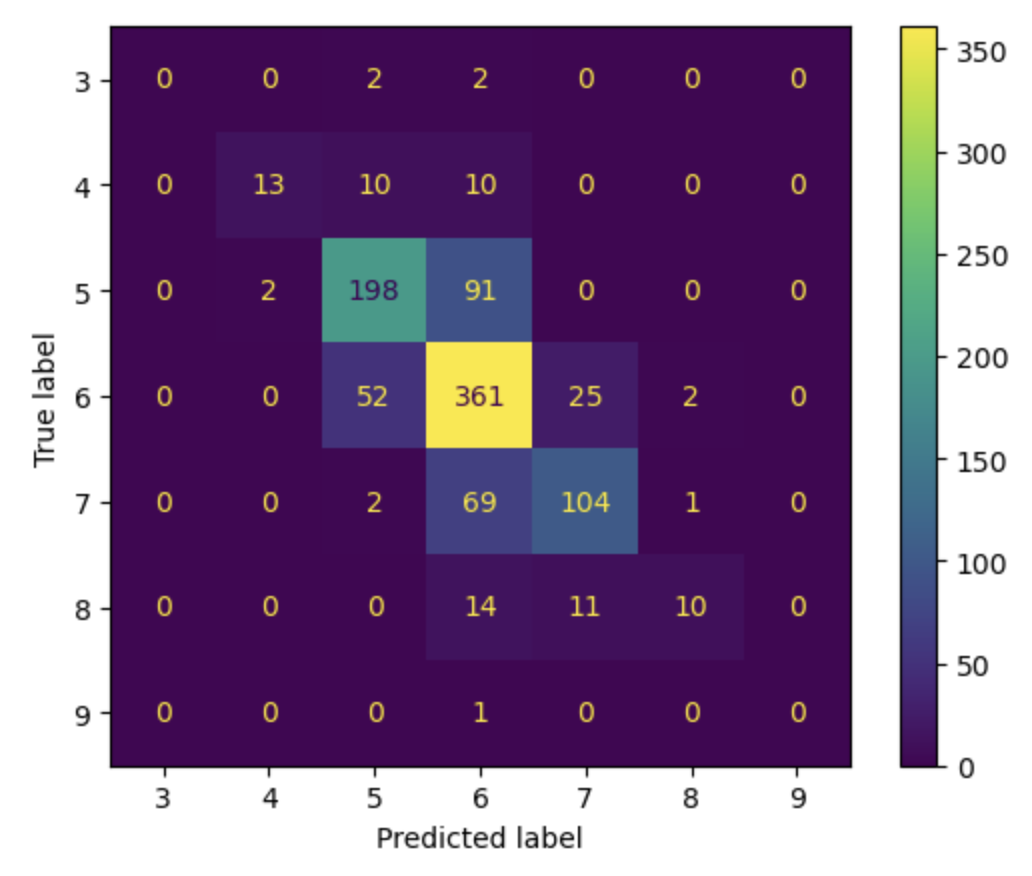
\includegraphics[width=.45\textwidth]{img/finalperform.png}
	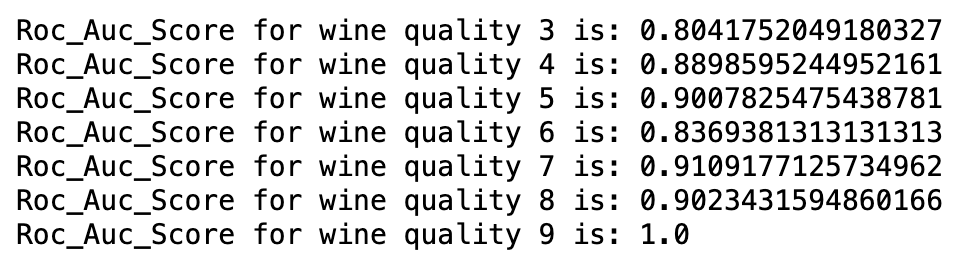
\includegraphics[width=.75\textwidth]{img/finalrocaucscore.png}
\end{center}

\begin{thebibliography}{9}
	\bibitem{dataset} A. Asuncion, D. Newman, UCI Machine Learning Repository, University of California, Irvine  (2007).  Obtained from https://archive-beta.ics.uci.edu/dataset/186/wine+quality. 
	\bibitem{numpyisnan} C. Harris, K. Millman, S. van der Walt,  Array programming with NumPy. Nature 585, 357–362 (2020). DOI: 10.1038/s41586-020-2649-2.  https://numpy.org/doc/stable/reference/generated/numpy.isnan.html
	\bibitem{seaborn} M. Waskom, (2021). seaborn: statistical data visualization. Journal of Open Source Software, 6(60), 3021, https://doi.org/10.21105/joss.03021.
	\bibitem{scikitlearn}Scikit-learn: Machine Learning in Python, Pedregosa et al., JMLR 12, pp. 2825-2830, 2011. 
	\bibitem{skopt} ScikitLearn-Optimizer. (2021). obtained from: https://scikit-optimize.github.io/stable/modules/generated/skopt.BayesSearchCV.html
\end{thebibliography}

\end{document}
